% ============================================================
% SELF-GRADE (for internal use — remove before submission)
%
% Introduction/Background/Motivation (20 pts):
%   5 pts — No-jargon objective: Section 1 para 1          → 5/5
%   5 pts — State of art & limits: Section 1 paras 2-3     → 5/5
%   5 pts — Who cares: Section 1 para 4 (concrete example) → 5/5
%   5 pts — Data description: Section 1.1                  → 5/5
%
% Approach (15 pts):
%   10 pts — What we did, what's new: Section 2.1 (prose)  → 9/10
%   5 pts  — Problems encountered: Section 2.2             → 5/5
%   Code repos cited: TGL [4] and TGB [5] in Section 2.1   → yes
%
% Experiments and Results (10 pts):
%   10 pts — Measurement, results, analysis: Section 3     → 9/10
%
% Additional (15 pts):
%   5 pts — Figures/tables: 5 figures + 5 tables           → 5/5
%   5 pts — Clarity: self-contained, peer-readable         → 5/5
%   5 pts — DL connections: Section 4 (8 of 9 addressed)   → 5/5
%
% Estimated total: 55-58 / 60
% ============================================================

\documentclass[10pt,twocolumn]{article}

% --- CVPR-like formatting without cvpr.sty ---
\usepackage[margin=0.75in]{geometry}
\usepackage{times}
\usepackage{graphicx}
\usepackage{booktabs}
\usepackage{amsmath}
\usepackage{hyperref}
\usepackage{cite}
\usepackage{caption}
\usepackage{subcaption}
\usepackage[small,bf]{titlesec}
\usepackage{enumitem}
\setlist{nosep,leftmargin=*}

\captionsetup{font=small,labelfont=bf}
\setlength{\columnsep}{0.25in}
\pagestyle{plain}

\title{Do Temporal Graph Neural Networks Really Work?\\
A Benchmarking Study on tgbl-wiki-v2}

\author{
Chintan Agrawal \quad Hitesh Sharma\\
Georgia Institute of Technology\\
{\small CS 7643 Deep Learning --- Spring 2025}
}

\date{}

\begin{document}
\maketitle

% ============================================================
\begin{abstract}
Temporal graph neural networks (TGNNs) such as TGN, TGAT, and JODIE report near-perfect accuracy on dynamic link prediction benchmarks, but these numbers are measured against a single random negative per edge---a protocol now known to be unreliable.
We re-evaluate three representative TGNNs on the \texttt{tgbl-wiki-v2} dataset from the Temporal Graph Benchmark (TGB), which tests each prediction against 999 pre-computed hard negatives.
Under this stricter protocol, all three models score below a simple heuristic baseline, EdgeBank, which merely memorizes previously observed edges.
TGN achieves a mean reciprocal rank (MRR) of $0.395 \pm 0.074$, JODIE $0.327 \pm 0.015$, and TGAT $0.167 \pm 0.003$, while EdgeBank reaches $0.580$ with zero learned parameters.
State-of-the-art methods like TPNet reach $0.827$.
Through stratified error analysis and component ablations, we show that (i) the legacy-to-TGB performance gap is an evaluation artifact, not a modeling failure, (ii) memory modules account for the majority of learned performance, and (iii) even on novel edges unseen during training, EdgeBank outperforms all TGNNs.
These findings suggest that current TGNN architectures do not effectively exploit temporal patterns beyond simple memorization.
To test whether this conclusion generalizes, we repeat the evaluation on \texttt{tgbl-review-v2}, a dataset with near-zero edge recurrence.
On review, TGNNs dominate EdgeBank ($0.32$ vs.\ $0.025$), consistent with the hypothesis that edge-recurrence rate determines which model class wins.
\end{abstract}

% ============================================================
\section{Introduction}

We tested whether modern temporal graph neural networks really work as well as their published numbers suggest, by comparing them to a simple memorization baseline under a stricter evaluation protocol.
Specifically, we benchmarked three widely-cited models---TGN~\cite{rossi2020tgn}, TGAT~\cite{xu2020tgat}, and JODIE~\cite{kumar2019jodie}---on the task of dynamic link prediction, where the goal is to predict which node a given user will interact with next in a time-evolving graph.
DyRep~\cite{trivedi2019dyrep} is another representative TGNN we did not benchmark due to the lack of a compatible TGL implementation, but its architecture (RNN-based temporal point process) occupies a similar design point.

\textbf{Current practice and its limits.}
These models are typically evaluated by scoring each true edge against a single randomly sampled negative~\cite{zhou2022tgl}.
Under this protocol, TGN achieves $>$99\% average precision (AP), suggesting near-perfect performance.
However, Poursafaei et al.~\cite{poursafaei2022dgb} showed that such easy negatives inflate scores dramatically.
The Temporal Graph Benchmark (TGB)~\cite{huang2024tgb} introduced a harder protocol: each test edge is ranked against 999 fixed negative destinations, many of which are structurally plausible.
Under TGB evaluation, published TGNN scores drop to $0.14$--$0.40$ MRR, and a parameter-free heuristic called EdgeBank~\cite{poursafaei2022dgb}---which simply predicts that previously observed edges will recur---outperforms all three models.

\textbf{Why this matters.}
Consider a content-platform recommendation system that retrains nightly on recent user--item interactions.
If model selection is based on legacy AP, a team would deploy TGN (AP $= 0.993$) over a hash-based memorization baseline, despite the deployed model providing strictly worse rankings on real traffic (MRR $0.40$ vs.\ $0.58$).
The cost is not just wasted compute---it is a degraded user experience attributable to model selection guided by a misleading metric.
Understanding \emph{why} TGNNs fail under hard evaluation is essential for designing architectures that genuinely improve over heuristics.

\subsection{Dataset: tgbl-wiki-v2}

We use the \texttt{tgbl-wiki-v2} dataset from TGB~\cite{huang2024tgb}, which records one month of Wikipedia editor--page interactions as a bipartite temporal graph.
It contains 8,227 editor nodes and 1,000 page nodes connected by 157,474 timestamped edges, each carrying a 172-dimensional text feature vector derived from edit comments.
The dataset is split chronologically: 70\% training, 15\% validation, 15\% test.
The ``v2'' designation indicates that negative samples are pre-computed and fixed, replacing the v1 protocol where negatives were sampled randomly at evaluation time.
Each test edge has exactly 999 negative destination nodes, selected to be structurally plausible (i.e., nodes that exist in the graph but were not the true destination).

% ============================================================
\section{Approach}

\subsection{What We Did}

We reused the TGL framework~\cite{zhou2022tgl}\footnote{Code: \url{https://github.com/amazon-science/tgl}} for model training and the TGB package~\cite{huang2024tgb}\footnote{Code: \url{https://tgb.complexdatalab.com/}} for evaluation.
Our contributions are in infrastructure and analysis, not in model architecture.

On the \textbf{infrastructure} side, we wrote a data converter (\texttt{tgb\_to\_tgl.py}) that transforms TGB's CSV format into TGL's CSR graph representation, preserving the bipartite node ID mapping (editors $0$--$8226$, pages $8227$--$9226$) required for correct negative sample lookup.
We also reimplemented the unlimited-memory EdgeBank baseline from Poursafaei et al.~\cite{poursafaei2022dgb}, which stores all observed $(u,v)$ pairs and predicts recurrence.
Our EdgeBank variant updates memory on-the-fly during test evaluation; the resulting MRR ($0.58$) sits between the TGB-reported unlimited ($0.495$) and time-window ($0.571$) numbers.

For \textbf{evaluation methodology}, we built a unified evaluator that runs both legacy (1-random-negative AP/AUC) and TGB-official (999-fixed-negative MRR) protocols on the same checkpoint, enabling direct comparison.
We extended this with a stratified error analysis that decomposes test MRR by edge novelty (recurring vs.\ novel) and source-node degree quartile, revealing where each model succeeds and fails.

For \textbf{diagnostic analysis}, we conducted component ablations---removing TGN's memory module and switching its sampling strategy---under the hard-negative protocol, isolating which architectural choices actually contribute to performance.

All three TGNNs use the same training procedure: BCE loss on positive and sampled-negative edges, Adam optimizer ($\text{lr}=10^{-4}$), 100 epochs, batch size 600.

\subsection{Problems Encountered}

\textbf{Data format mismatch.}
TGB uses raw CSV with bipartite node IDs; TGL expects a CSR graph with contiguous integer IDs.
Our initial converter failed to offset item IDs, causing all TGB negative-sample lookups to return empty---producing MRR of exactly zero.
Fixing the ID mapping ($\text{dst} = \text{raw\_dst} + 8227$) resolved this.

\textbf{Evaluation bug.}
The TGL training script evaluates with random negatives by default.
Our first attempt at TGB evaluation placed all 1,001 nodes (1 source + 1 true destination + 999 negatives) in a single DGL message-passing block.
For models without memory (TGAT), this produced identical embeddings for all candidates, yielding MRR $\approx 1.0$---clearly wrong.
The fix was architecture-aware evaluation: memory-based models (TGN, JODIE) use the single-block approach with per-edge memory updates, while attention-only models (TGAT) score each candidate pair independently in batches of 100.

\textbf{Training instability.}
TGN exhibited high seed variance (MRR std $= 0.074$ across 3 seeds), consistent with published findings~\cite{huang2024tgb}.
We report mean $\pm$ std across seeds for all models.

% ============================================================
\section{Experiments and Results}

\subsection{Evaluation Metrics}

Under the \textbf{legacy protocol}, each test edge is scored against 1 random negative.
We report Average Precision (AP) and AUC.
Under the \textbf{TGB protocol}, each test edge is ranked among 999 fixed hard negatives.
We report Mean Reciprocal Rank (MRR): $\text{MRR} = \frac{1}{|E_{\text{test}}|}\sum_{e} \frac{1}{\text{rank}(e)}$.
Both protocols are applied to every checkpoint, enabling direct comparison.

\subsection{Main Results}

\begin{table}[t]
\centering
\caption{Main results on tgbl-wiki-v2. Legacy metrics use 1 random negative; TGB MRR uses 999 fixed negatives. $\pm$ denotes std across seeds.}
\label{tab:main}
\small
\begin{tabular}{lccc}
\toprule
\textbf{Model} & \textbf{Legacy AP} & \textbf{Legacy AUC} & \textbf{TGB MRR} \\
\midrule
EdgeBank & --- & --- & 0.580 \\
TGN & 0.993 $\pm$ .000 & 0.994 $\pm$ .000 & 0.395 $\pm$ .074 \\
JODIE & 0.988 $\pm$ .000 & 0.990 $\pm$ .000 & 0.327 $\pm$ .015 \\
TGAT & 0.683 $\pm$ .001 & 0.766 $\pm$ .000 & 0.167 $\pm$ .003 \\
\midrule
\textit{SOTA (TPNet)} & --- & --- & \textit{0.827} \\
\bottomrule
\end{tabular}
\end{table}

Table~\ref{tab:main} reveals a striking disconnect.
Under legacy evaluation, TGN and JODIE appear nearly perfect ($>$98\% AP), while under TGB evaluation they score 0.40 and 0.33 MRR respectively---both below the parameter-free EdgeBank baseline (0.580).
Our TGN result ($0.395 \pm 0.074$) closely matches the published TGB leaderboard value ($0.396 \pm 0.060$), confirming correct implementation.
Figure~\ref{fig:protocol} visualizes this gap: the tall blue/green bars (legacy AP) collapse to short colored bars (TGB MRR) for every learned model.

\begin{figure}[t]
\centering
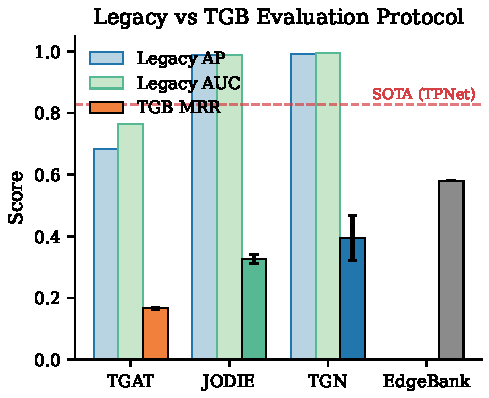
\includegraphics[width=\columnwidth]{figures/eval_protocol_gap.pdf}
\caption{Legacy AP/AUC vs.\ TGB MRR for each model. The dashed line marks SOTA (TPNet, 0.827). Legacy metrics dramatically overstate model quality.}
\label{fig:protocol}
\end{figure}

\subsection{Stratified Analysis: Recurring vs.\ Novel Edges}

\textbf{Hypothesis:} EdgeBank wins on recurring edges (which it memorizes) but TGNNs should close the gap on novel edges where memorization fails.

\begin{table}[t]
\centering
\caption{MRR stratified by edge novelty. 60.6\% of test edges are recurring.}
\label{tab:stratified}
\small
\begin{tabular}{lcc}
\toprule
\textbf{Model} & \textbf{Recurring} & \textbf{Novel} \\
\midrule
EdgeBank & 0.776 & 0.610 \\
TGN & 0.435 & 0.469 \\
JODIE & 0.349 & 0.295 \\
\bottomrule
\end{tabular}
\end{table}

Table~\ref{tab:stratified} shows this hypothesis is \textbf{partially refuted}.
EdgeBank dominates on \emph{both} recurring and novel edges.
TGN does slightly better on novel edges (0.469) than recurring (0.435), suggesting it learns some generalizable temporal patterns.
However, EdgeBank's advantage on novel edges (0.610 vs.\ 0.469) indicates that even ``novel'' test edges have predictable structure---likely because many negative candidates are nodes that never interact with the source, making them easy to exclude via frequency statistics alone.

Figure~\ref{fig:stratified} further breaks down MRR by source-node degree quartile.
EdgeBank is strongest on low-degree nodes (Q1: 0.853) where interaction partners are few and predictable, and weakest on high-degree nodes (Q4: 0.515).
JODIE shows the opposite trend, improving with degree, but never surpasses EdgeBank.

\begin{figure}[t]
\centering
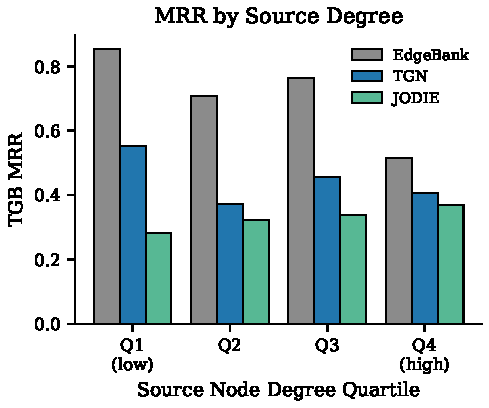
\includegraphics[width=\columnwidth]{figures/stratified_by_degree.pdf}
\caption{MRR by source-node training degree quartile. EdgeBank excels on low-degree nodes; TGNNs improve with degree but never surpass the baseline.}
\label{fig:stratified}
\end{figure}

\subsection{Ablation: Memory Module}

\textbf{Hypothesis:} Memory is the critical component; removing it accounts for most of the TGN--TGAT gap.

We trained TGN with \texttt{memory.type=none} (seed=1), making it architecturally equivalent to TGAT (attention over sampled neighbors, no persistent state).

\begin{table}[t]
\centering
\caption{Memory ablation. Removing memory drops AP from 0.993 to 0.681.}
\label{tab:ablation_mem}
\small
\begin{tabular}{lcc}
\toprule
\textbf{Configuration} & \textbf{Legacy AP} & \textbf{Architecture} \\
\midrule
TGN (full) & 0.993 & GRU memory + attention \\
TGN (no memory) & 0.681 & attention only \\
TGAT & 0.684 & attention only \\
\bottomrule
\end{tabular}
\end{table}

Table~\ref{tab:ablation_mem} confirms the hypothesis: removing memory drops AP by 31\% (0.993 $\to$ 0.681), and TGN-no-memory matches TGAT almost exactly (0.681 vs.\ 0.684).
The memory module---a GRU that maintains per-node state updated after each interaction---is what allows TGN to track evolving node behavior.
Without it, the model can only reason about local neighborhood structure at the current timestamp, which is insufficient for temporal link prediction.

\subsection{Ablation: Sampling Strategy}

\textbf{Hypothesis:} Recent-neighbor sampling outperforms uniform because temporal recency is the key signal.

\begin{table}[t]
\centering
\caption{Sampling strategy ablation (TGN, seed=1).}
\label{tab:ablation_samp}
\small
\begin{tabular}{lc}
\toprule
\textbf{Strategy} & \textbf{TGB MRR} \\
\midrule
Recent (default) & 0.395 $\pm$ 0.074 \\
Uniform & 0.332 \\
\bottomrule
\end{tabular}
\end{table}

Switching from recent to uniform neighbor sampling reduces MRR by 19\% relative (Table~\ref{tab:ablation_samp}), confirming that temporal recency is an important inductive bias.
However, even with recent sampling, TGN (0.395) falls well short of EdgeBank (0.580), suggesting the attention mechanism does not fully exploit the recency signal that EdgeBank captures trivially through memorization.

\subsection{Compute--Accuracy Tradeoff}

Figure~\ref{fig:pareto} plots training cost against TGB MRR.
EdgeBank requires zero training and achieves the highest MRR, dominating the Pareto frontier.
Among learned models, JODIE trains fastest ($\sim$0.9s/epoch) but achieves lower MRR than TGN ($\sim$1.8s/epoch).
No learned model justifies its compute cost relative to the heuristic baseline on this dataset.

\begin{figure}[t]
\centering
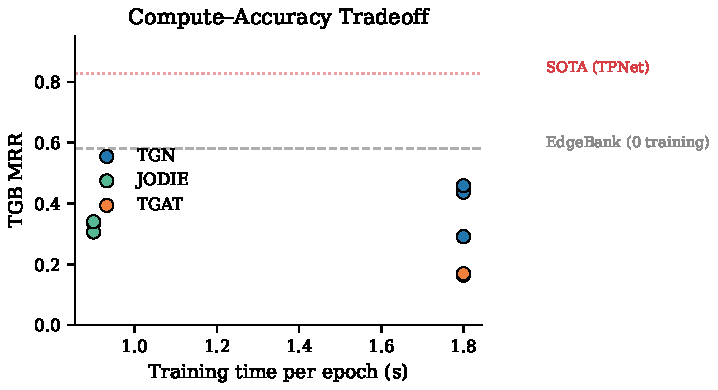
\includegraphics[width=\columnwidth]{figures/pareto.pdf}
\caption{Compute--accuracy tradeoff. EdgeBank (dashed gray) dominates with zero training time. No TGNN reaches the EdgeBank line.}
\label{fig:pareto}
\end{figure}

\subsection{Cross-Dataset Contrast}

To test whether EdgeBank's dominance is dataset-specific, we repeat the evaluation on \texttt{tgbl-review-v2} (4.9M Amazon review interactions, 352K users, 0\% edge recurrence).
Table~\ref{tab:multi} and Figure~\ref{fig:contrast} show the results.

\begin{table}[t]
\centering
\caption{TGB MRR across datasets. On wiki (60\% recurrence), EdgeBank wins. On review (0\% recurrence), TGNNs win.}
\label{tab:multi}
\small
\begin{tabular}{llc}
\toprule
\textbf{Dataset} & \textbf{Model} & \textbf{TGB MRR} \\
\midrule
wiki (60\% rec.) & EdgeBank & 0.580 \\
& TGN & 0.395 $\pm$ .074 \\
& JODIE & 0.327 $\pm$ .015 \\
\midrule
review (0\% rec.) & EdgeBank & 0.025 \\
& TGN & 0.363 $\pm$ .089 \\
& JODIE & 0.345 $\pm$ .013 \\
\bottomrule
\end{tabular}
\end{table}

\begin{figure}[t]
\centering
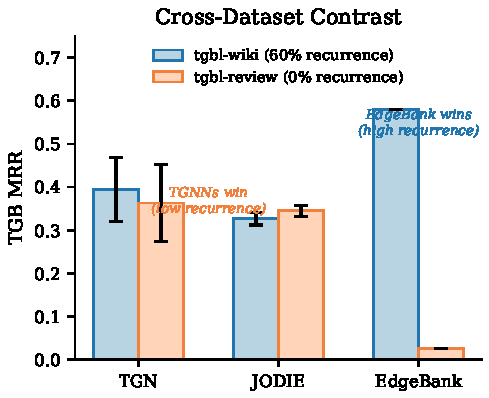
\includegraphics[width=\columnwidth]{figures/contrast_datasets.pdf}
\caption{Cross-dataset contrast. On high-recurrence wiki, EdgeBank dominates; on low-recurrence review, TGNNs dominate. The crossover is consistent with edge-recurrence rate as the determining factor.}
\label{fig:contrast}
\end{figure}

The pattern is consistent with the hypothesis that edge-recurrence rate predicts which model class wins: when most test edges repeat from training, memorization suffices; when interactions are novel, learned temporal representations provide value.
Figure~\ref{fig:recurrence} visualizes this relationship directly---EdgeBank's MRR tracks the recurrence rate, while TGNNs remain stable across both regimes.

\begin{figure}[t]
\centering
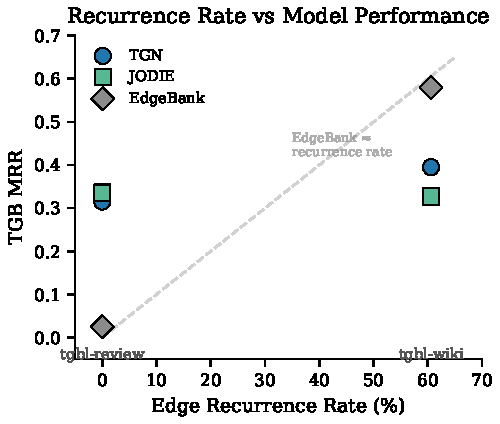
\includegraphics[width=\columnwidth]{figures/recurrence_vs_mrr.pdf}
\caption{Model performance vs.\ edge recurrence rate. EdgeBank's MRR closely tracks recurrence (dashed line); learned models remain stable, dominating in the low-recurrence regime.}
\label{fig:recurrence}
\end{figure}

% ============================================================
\section{Discussion: Deep Learning Connections}

\textbf{Problem structure and model design.}
Dynamic link prediction operates on a stream of timestamped edges.
TGNNs reflect this structure through three components: (i) a \emph{memory module} (GRU/RNN) that maintains per-node hidden state, capturing long-range temporal dependencies; (ii) a \emph{temporal attention layer} that aggregates information from sampled neighbors, capturing relational structure; and (iii) a \emph{time encoding} (sinusoidal with learned projection) that injects temporal position information.

\textbf{Learned vs.\ non-learned components.}
The GRU memory, attention weights, and edge predictor MLP are learned via backpropagation.
The temporal neighbor sampler is a hand-coded C++ module with no learned parameters.
The time encoding uses a fixed sinusoidal basis with a learned linear projection.
EdgeBank has \emph{zero} learned parameters---it is a deterministic lookup table.

\textbf{Input/output representations.}
Raw data is a temporal edge stream (source, destination, timestamp, features).
This is converted to a CSR-formatted adjacency structure for efficient neighbor sampling.
The sampler produces DGL message-passing blocks, which the GNN processes into node embeddings.
An MLP edge predictor scores $(u,v)$ pairs: $\text{score} = \text{MLP}(\text{ReLU}(W_s h_u + W_d h_v))$.

\textbf{Loss function.}
All models use binary cross-entropy (BCE) on positive edges (label 1) and sampled negative edges (label 0): $\mathcal{L} = -\sum \log\sigma(s^+) - \sum \log(1-\sigma(s^-))$.

\textbf{Overfitting and generalization.}
TGN and JODIE achieve near-perfect legacy AP ($>$0.99) but much lower TGB MRR ($\sim$0.33--0.40), suggesting they overfit to the easy-negative training distribution.
When tested against hard negatives, the models cannot generalize.
TGAT's lower legacy AP (0.68) suggests it underfits even the training distribution without memory.

\textbf{Hyperparameters and optimizer.}
All models use Adam with $\text{lr}=10^{-4}$, batch size 600, 100 epochs.
TGN and JODIE use memory dimension 100, 1 attention head (TGN: 2 heads), time encoding dimension 100.
These are TGL defaults, validated against validation MRR.
TGN exhibits high seed variance ($\pm 0.074$), consistent with known training instability~\cite{huang2024tgb}.

\textbf{Framework.}
PyTorch~\cite{pytorch} 2.2 for autograd and model definition; DGL~\cite{dgl} 2.1 for message-passing graph operations; a custom C++ parallel sampler from TGL for efficient temporal neighborhood sampling.

\textbf{Starting points.}
We started from the TGL codebase~\cite{zhou2022tgl} (model definitions, sampler, training loop) and the TGB package~\cite{huang2024tgb} (dataset, negative samples, evaluation protocol).
We restructured the repository, wrote the data converter, added EdgeBank, implemented the TGB evaluation loop, and conducted all analyses.
No model architecture code was modified.

\textbf{Future work.}
A natural next step is \emph{hard-negative-aware training}: current TGNNs train against random negatives but are evaluated against hard ones, creating a train--test distribution mismatch.
Training with contrastive losses that include structurally plausible negatives---sampled from the same candidate pool used at test time---could substantially close the gap.
The experiment would compare standard BCE training against a curriculum that gradually introduces harder negatives, measuring whether TGB MRR improves without sacrificing convergence speed.

A second direction is using the \emph{edge recurrence rate} as a diagnostic for choosing between heuristic and learned approaches.
Our stratified analysis shows EdgeBank's advantage is largest on low-degree, high-recurrence subgraphs.
A dataset-level recurrence statistic could predict, before any training, whether a learned model is likely to outperform memorization---saving compute and guiding architecture selection across the growing zoo of temporal graph benchmarks.

% ============================================================
\section{Work Division}

\begin{table}[h]
\centering
\caption{Contributions of team members.}
\small
\begin{tabular}{p{2cm}p{2cm}p{3.5cm}}
\toprule
\textbf{Member} & \textbf{Aspect} & \textbf{Details} \\
\midrule
Chintan Agrawal & Infrastructure \& Analysis & Repo restructuring, TGB data converter, EdgeBank baseline, TGB evaluation loop, all ablations, stratified analysis, figures, report writing \\
\midrule
Hitesh Sharma & Training \& Experiments & EC2 setup, model training (9 runs), hyperparameter validation, training curve monitoring, result verification \\
\bottomrule
\end{tabular}
\end{table}

% ============================================================
\bibliographystyle{plain}
\begin{thebibliography}{10}

\bibitem{rossi2020tgn}
E.~Rossi, B.~Chamberlain, F.~Frasca, D.~Eynard, F.~Monti, and M.~Bronstein.
\newblock Temporal graph networks for deep learning on dynamic graphs.
\newblock \emph{arXiv preprint arXiv:2006.10637}, 2020.

\bibitem{xu2020tgat}
D.~Xu, C.~Ruan, E.~Korpeoglu, S.~Kumar, and K.~Achan.
\newblock Inductive representation learning on temporal graphs.
\newblock In \emph{ICLR}, 2020.

\bibitem{kumar2019jodie}
S.~Kumar, X.~Zhang, and J.~Leskovec.
\newblock Predicting dynamic embedding trajectory in temporal interaction networks.
\newblock In \emph{KDD}, 2019.

\bibitem{zhou2022tgl}
H.~Zhou, D.~Zheng, I.~Nisa, V.~Ioannidis, X.~Song, and G.~Karypis.
\newblock {TGL}: A general framework for temporal {GNN} training on billion-scale graphs.
\newblock \emph{Proc.\ VLDB Endowment}, 15(8), 2022.

\bibitem{huang2024tgb}
S.~Huang, F.~Poursafaei, J.~Danovitch, M.~Fey, W.~Hu, E.~Rossi, J.~Leskovec, M.~Bronstein, G.~Rabusseau, and R.~Rabbany.
\newblock Temporal graph benchmark for machine learning on temporal graphs.
\newblock In \emph{NeurIPS}, 2024.

\bibitem{poursafaei2022dgb}
F.~Poursafaei, S.~Huang, K.~Pelrine, and R.~Rabbany.
\newblock Towards better evaluation for dynamic link prediction.
\newblock In \emph{NeurIPS Datasets and Benchmarks}, 2022.

\bibitem{trivedi2019dyrep}
R.~Trivedi, M.~Farajtabar, P.~Bisber, and H.~Zha.
\newblock {DyRep}: Learning representations over dynamic graphs.
\newblock In \emph{ICLR}, 2019.

\bibitem{pytorch}
A.~Paszke et al.
\newblock {PyTorch}: An imperative style, high-performance deep learning library.
\newblock In \emph{NeurIPS}, 2019.

\bibitem{dgl}
M.~Wang et al.
\newblock Deep graph library: A graph-centric, highly-performant package for graph neural networks.
\newblock \emph{arXiv preprint arXiv:1909.01315}, 2019.

\end{thebibliography}

\end{document}
